\documentclass{article} 
\usepackage[left=0.75in,top=0.6in,right=0.75in,bottom=0.6in]{geometry} % Document margins
\usepackage{tabularx}
\usepackage{fancyvrb}
%\usepackage[hidelinks]{hyperref}
\usepackage{graphicx}


\begin{document}

%----------------------------------------------------------------------------------------
%		 TITLE PAGE
%----------------------------------------------------------------------------------------

\begin{titlepage}

\vspace*{45 pt}
\begin{center}
\Huge{\bf CS 432/532:  Web Science}\\
\huge{Spring 2017\\}

\vspace{60 pt}
\Huge\underline {Assignment 1}\\

\vspace{10 pt}
\Huge{Michael Micros}\\\

\vspace{200 pt}
{\huge \bf {Honor Pledge}}\\
\Large{I pledge to support the Honor System of Old Dominion University. I will refrain from any form of academic dishonesty or deception, such as cheating or plagIiarism. I am aware that as a member of the academic community it is my responsibility to turn in all suspected violations of the Honor Code. I will report to a hearing if summoned. }\\
\vspace {.5cm}

{Signed \_\_\_\_\_\_\_\_\_\_\_\_\_\_\_\_\_\_\_\_\_\_\_\_\_\_\_\_\_\_\_\_\_\_}\\
\today

\end{center}
\end{titlepage}




%----------------------------------------------------------------------------------------
%		PROBLEM 1
%----------------------------------------------------------------------------------------

\section*{\underline{Problem 1}}

\subsection*{Question}

\begin{verbatim}
1.  Demonstrate that you know how to use "curl" well enough to
correctly POST data to a form.  Show that the HTML response that
is returned is "correct".  That is, the server should take the
arguments you POSTed and build a response accordingly.  Save the
HTML response to a file and then view that file in a browser and
take a screen shot.

\end{verbatim}

\subsection*{Answer}


\begin{verbatim}
In order to answer this question, all that was necessary was to read through 
the curl command manual, which is found by typing "man curl" into the command line.
The exact command used was "curl -v -d" as can be seen in Fig. 1.
Option "-v" makes curl verbose during the operation.
Option "-d <data>" sends the data as a POST request to the HTTP server.
Finally, the form to which the data was POSTed was found from a website that 
allows the user to POST and inspect the generated response as seen in Fig. 2. 

\end{verbatim}

\begin{figure}[ht!]
\centering
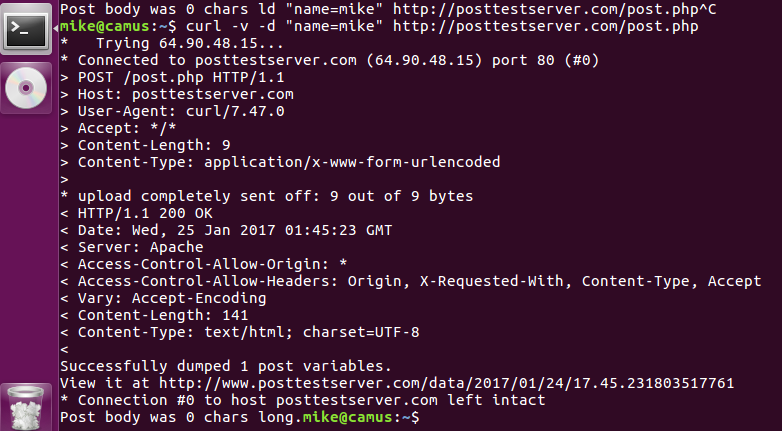
\includegraphics[width=\linewidth]{curl.png}
\caption{curl command in terminal \label{overflow}}
\end{figure}

\newpage

\begin{center}
\begin{figure}[ht!]
\centering
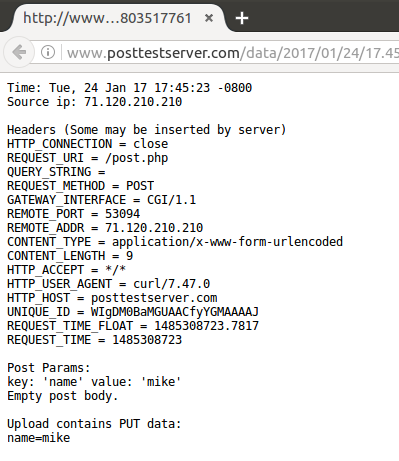
\includegraphics[width=300 px]{HTMLresponse.png}
\caption{HTML responsel \label{overflow}}
\end{figure}
\end{center}

\newpage


%----------------------------------------------------------------------------------------
%		PROBLEM 2
%----------------------------------------------------------------------------------------

\section*{\underline{Problem 2}}

\subsection*{Question}

\begin{verbatim}
2.  Write a Python program that:
  1. takes as a command line argument a web page
  2. extracts all the links from the page
  3. lists all the links that result in PDF files, and prints out
     the bytes for each of the links.  (note: be sure to follow
     all the redirects until the link terminates with a "200 OK".)
  4. show that the program works on 3 different URIs, one of which
     needs to be: 
     http://www.cs.odu.edu/~mln/teaching/cs532-s17/test/pdfs.html
\end{verbatim}

\subsection*{Answer}


\begin{verbatim}
1. In order  for our Python program to accept a command line argument, 'sys' must be imported. 
This allows us to access the arguments that are entered at the command line. "argv[0]" is the 
command that executes the python script and "argv[1]" is the web page that the user selected.

2. After the desired web page was opened using "urllib.request.openurl() ", Beautifulsoup was
used to parse all the links on the page using the instructions: 
        >>>  soup = BeautifulSoup(Html,"html.parser")
        >>> for link in soup.find_all('a'):

3. In order to detect the content type of each link, a new request was made for each link obtained 
in the previous part. Using urllib we are able to search the info of the response to check if the
response code was "200 OK" and whether the "Content-type" was "application/pdf". I specifically 
searched the content type for anyninstance of the string "pdf" because there are cases where the 
content is of type PDF but the notation is slightly different than the standard. The instruction 
that does all this is: 
         >>>if('pdf' in linkRes.info()['Content-Type'] and (linkRes.code== 200) ):

4.The results of the program can be seen in Figure 4 and 5.
\end{verbatim}

\begin{figure}[ht!]
\centering
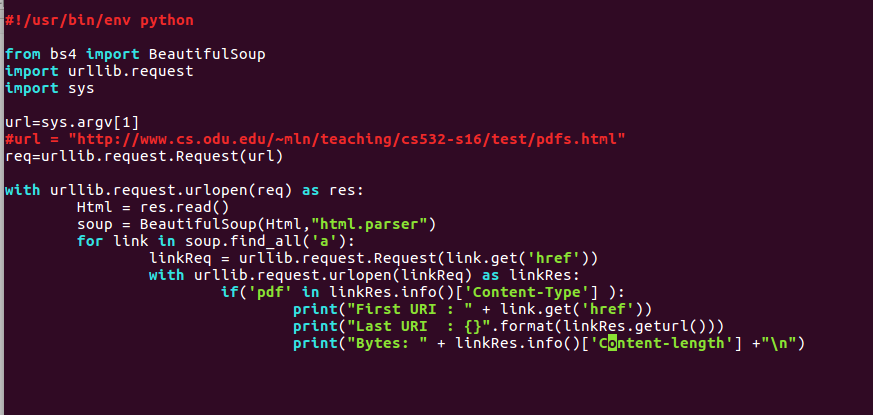
\includegraphics[width=\linewidth]{p2_code.png}
\caption{p2.py (Located in Problem2 directory) \label{overflow}}
\end{figure}

\begin{figure}[ht!]
\centering
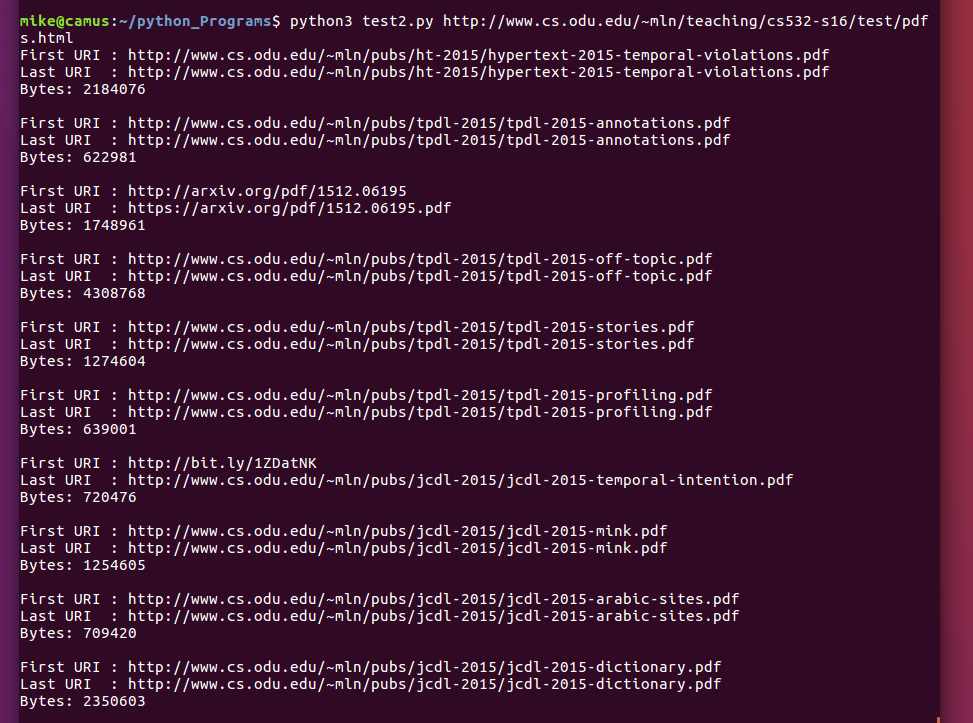
\includegraphics[width=\linewidth]{p2_result.png}
\caption{p2.py (Result for http://www.cs.odu.edu/~mln/teaching/cs532-s17/test/pdfs.html ) \label{overflow}}
\end{figure}



\begin{figure}[ht!]
\centering
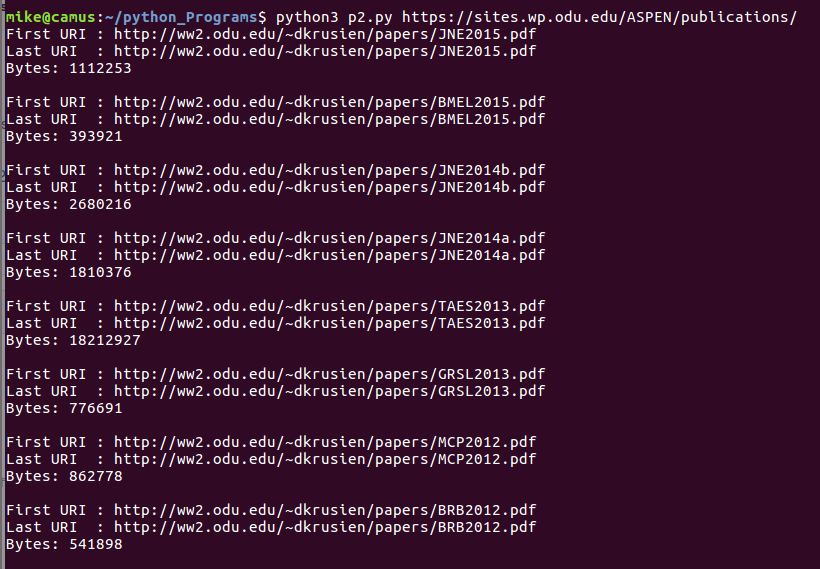
\includegraphics[width=\linewidth]{p2_result2.png}
\caption{p2.py (Result for https://sites.wp.odu.edu/ASPEN/publications/) \label{overflow}}
\end{figure}



%----------------------------------------------------------------------------------------
%		PROBLEM 3
%----------------------------------------------------------------------------------------

\section*{\underline{Problem 3}}

\subsection*{Question}

\begin{verbatim}

3.  Consider the "bow-tie" graph in the Broder et al. paper (fig 9):
    http://www9.org/w9cdrom/160/160.html

    Now consider the following graph:

    A --> B
    B --> C
    C --> D
    C --> A
    C --> G
    E --> F
    G --> C
    G --> H
    I --> H
    I --> K
    L --> D
    M --> A
    M --> N
    N --> D
    O --> A
    P --> G 
    
    For the above graph, give the values for:

    IN: 
    SCC: 
    OUT: 
    Tendrils: 
    Tubes: 
    Disconnected:

\end{verbatim}

\subsection*{Answer}


\begin{verbatim}
After mapping out the graph that was given (the Figure below), it becomes evident 
which are the inputs, outputs and strongly connected components. The components
 of the graph that are not pointed(linked) to by other componentss and have at least 
one connection to the SCC are  INPUTS . The components that do not point to anything 
but are pointed(linked) to by at least one component in the SCC  are OUTPUTS. The 
components that are all interconnected form the SCC area.The  nodes that do not connect 
to any of the other components are DISCONNECTED. Finally the nodes that connect only 
to the IN or OUT of the graph without connecting to the SCC are the TENDRILS. 


    IN: 	M,O,P
    SCC:  A,B,C,G
    OUT:  H,D
    Tendrils: I,K,L
    Tubes: N
    Disconnected: E,F

\end{verbatim}


\begin{figure}[ht!]
\centering
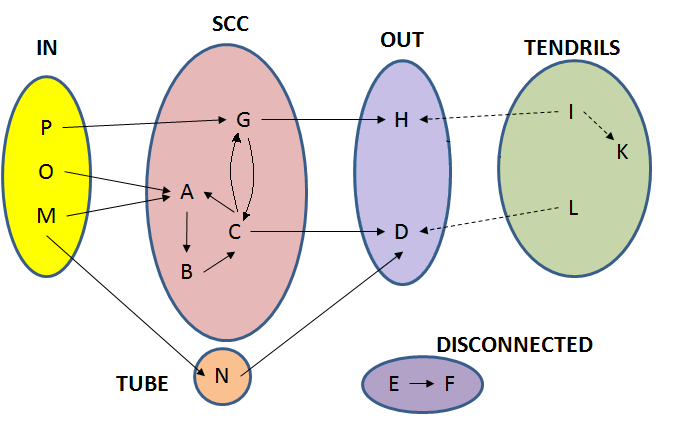
\includegraphics[width=\linewidth]{BowTie.png}
\caption{Bow Tie Graph \label{overflow}}
\end{figure}




%----------------------------------------------------------------------------------------
\end{document}
